\chapter{Concept}\label{sec:concept}
Based on the findings in Section~\ref{sec:analysis} we specify a formal language and a conceptual framework for \cmvs{} in this section.
Our approach involves the definition of the terminology and the basic components of the conceptual framework.
The first component is the shared data model on which all visualizations must agree on.
We formalize each interaction from Section~\ref{sec:analysis} as a mathematical function and group these functions together if they have the same input and output.
As a last step, we specify the communication pattern of the formalized language.

\section{Terminology}
We introduce a couple of new terms in order to give a formal definition of the conceptual framework

\textbf{Trigger} describes the event that starts an interaction.
As we have seen in Section~\ref{sec:analysis} every interaction is started by a user action.
The user e.g.\ clicks on a shape in the view, hovers over an area, selects an item from a dropdown menu, turns around a mobile device, speaks into the microphone or makes a particular gesture.
If the event of action is handled by a view and causes an interaction, we call this handling a \emph{trigger}.
Every view is responsible of its \emph{triggers}.
These are implementation details and are not shared by other views.

\textbf{Effect} is the change of the visual representation subsequent to the interaction.
In order to be perceivable by the user, the interaction must have some visual effect, i.e.\ a change in the visual representation of the data.
Examples are:
A change of colour of a selected bubble, a movement of the viewpoint, a rearrangement of attributes in a parallel plot or a higher level of detail in a \tmap{}.
Every view is responsible of its visual \emph{effects}.
Those are implementation details as well and they are not shared by other views.
Obviously visual effects are not shared, as it depends on the visualization if visual variables are constrained or available to express a visual effect.

In singular visualizations, interactions consist of at least of a trigger and an effect:
\begin{equation}
  I(T, E)
\end{equation}
The meaning of the interaction in a singular view can be implicit.
E.g.\ hovering over a geographic area changes the background colour of the polygon and the user can identify the interaction as a \emph{highlighting}.
Note that this implicit meaning must be explicit in \cmvs{} so that other views are able to process it.


\textbf{Subject} refers to the target of the interaction.
We must define what data or meta-data is affected by the interaction.
E.g.\ when a user moves the mouse cursor on a line in the line diagram, that could highlight the \emph{data point} under the cursor as well as the entire \emph{data series}.
Therefore we call the object affected of an interaction the interaction \emph{subject}.
A subject can be a data point, a list of data points, a position of the viewpoint, a certain order of attributes or a mapping of attributes to visual variables.

\textbf{Verb} refers to the application specific context and purpose of the interaction.
A developer may want to have many \emph{select} interactions.
E.g.\ the user desires to select a detail view of an item under the mouse cursor from a previously selected set of already highlighted items.
Therefore we allow for a user-defined \emph{verb}.
The verb describes the interaction in the context of a task or an intention that is intrinsic to the application the interaction happens in.

\textbf{Interaction function} is the declaration and definition how the subject of the interaction should be changed.
The aforementioned explicit meaning of the interaction is the smallest unit of information of the interaction.
This meaning is shared among multiple views, it is agnostic of how the interaction is implemented.
Therefore the meaning is shared between multiple views.
We call this meaning the \emph{interaction type}.
Some examples of interaction types include: Selection, Deletion, Point-of-Interest, Filtering, Reordering, Re-encoding.
Interaction types can be classified with the interaction categories of \textcite{Yi2007}.

Note that different information visualizations implement an interaction types in a different way or maybe not at all:

E.g.\ a bubble chart might encode a certain data attribute to the colour of a bubble.
Therefore the colour would not be changed for an interaction of type \emph{Selection} but the texture of the bubble.

A user may perform an interaction of type \emph{Reordering} on the series of a stacked bar chart.
This can have no effect on a coordinated scatter plot, as the position of each data point depends on its dimension.

\textbf{Sentence} is the minimal set of information to coordinate an interaction across multiple views.
We define a sentence $S$ as:
\begin{equation}
    S(V, F(IS))
\end{equation}
With $V$ as a verb, an interaction function $F$ and the interaction subject $IS$.
See Section~\ref{sec:concept:types} for a list of interaction functions.
A sentence contains everything necessary to ensure the interaction can be reflected in another view.

\textbf{Application context} is name for the state which is exclusive to the specific application.
Part of the application context is the access to data sources and the procedure to initialize data visualization with it.
Also, the binary files of textures, icons and vectors that describe the visual representation of a shape and colour themes are part of the application context.

\section{Formalization of an interaction}

We formalize an interaction $I$ as follows:
\begin{equation}
  I(T, S(V, F(IS)), E)
\end{equation}
For a trigger $T$, a sentence $S$ and the effect $E$.
The sentence $S$ is composed of a verb $V$, an interaction function definition $F$ and an interaction subject $IS$.
The part of the interaction which is shared among multiple views is the sentence $S$.
The function definition $F$ is defined by the triggering view at runtime.
E.g.\ when a parallel plot rearranges the list of attributes, the exact order will be determined by the view itself, during the handling of the drag-and-drop action.

\section{Conceptual Framework}
\todo[inline]{no section without text}

\section{Shared data model}\label{sec:concept:data-model}
To account for the various data structures, we use an abstract data model that is powerful enough to include tabular, hierarchical and relational data.
You can see a class diagram in figure~\ref{fig:concept:shared-data-model}.

The \emph{entity} class is used to model the smallest distinguishable unit.
All entities can be identified and retrieved via the \emph{id}.
An entity is defined to be any object that can have data attributes attached as \emph{dimensions}.

While entities describe what an object \emph{is}, a \emph{dimension} describes what it \emph{has}.

An entity can have arbitrary many attributes and each value can be accessed by the name of the attribute.
So if you want to get the \emph{latitude} value of an entity, you can retrieve the value with a call to the dimension \emph{latitude}.

Entities can also be \emph{series} of other entities.
A series contains an ordered list of contained entities.
As series can also contain other series, so we can model a hierarchy relation.

Every entity has a \emph{parent} which is the series it is contained in.
The root entity of the hierarchy has a parent which is \attr{nil}.
Every series has a special attribute \attr{height} that describes the number of nested series or the height of the subtree.

If we just want to display tabular data, we just have one or two levels of hierarchy.
E.g.\ one level of hierarchy for a histogram and two levels of hierarchy for a stacked bar chart.

Other relations than hierarchical relations can be modeled as a \emph{relation} entity.
It represents a directed edge in a graph and must have incoming and outgoing entity.
Since every \emph{relation} is an \emph{entity} as well, we can add \emph{attributes} to the relation.
These attributes may describe e.g.\ the weight of an edge in a flow map.


\begin{figure}[ht]
  \centering
  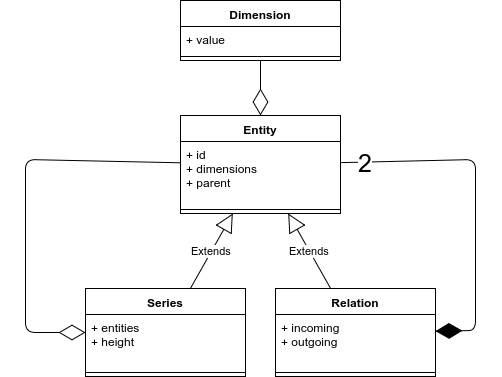
\includegraphics[width=0.5\textwidth]{images/concept/shared-data-model.png}
  \caption{%
    A data structure for tabular, hierarchical and relational data
  }\label{fig:concept:shared-data-model}
\end{figure}

\section{Predefined Interaction Functions}\label{sec:concept:types}

It turns out that we can describe the types of an interaction as a mathematical function.
These functions operates on the ids of \emph{entities}, \emph{series}, and \emph{relations} or their respective \emph{attributes}.
The name of the function is the \emph{type} of the interaction and the function domain being the \emph{subject} of the interaction.
Thus, we can describe interaction through a change of its semantic but we ignore implementation details of specific visualizations.


These function are derived from specific interactions of the examples in Section~\ref{sec:analysis}.
Domain and range of these functions refer to the objects defined in the data model in Section~\ref{sec:concept:data-model}.
To declare the functions explicitly, we define a couple of sets:

\begin{equation} \mathbb{E} : \mathbb{E} \subseteq \mathbb{N}  \end{equation}
  The set of all entities in our subject space.
  Each entity can be represented by its \attr{id}, so for simplicity $\mathbb{E}$ is a subset all natural numbers in $\mathbb{N}$.

\begin{equation} \mathbb{D} : \mathbb{D} \subseteq \Sigma^* \end{equation}
  The set of all dimensions in our shared data model.
  Dimensions of a data set are the attributes of our data model and both terms are used synonymously in the following.

\begin{equation} Space(\mathbb{D}) \end{equation}
  Where $Space$ is the range of values of a dimension $d \in \mathbb{D}$.

  For convenience, we define this set with a function $Space$ which maps the name of a dimension $d$ to its set of possible data values.
  So for an attribute \attr{name} that would be the set of all strings.
  For continuous values, that would be the set of all real numbers $\mathbb{R}$.
  But $Space(D)$ also includes the set of all possible discrete values of dimension. 

\begin{equation} \mathbb{V} = \{x,y,y2,y3\ldots{}yn,z,height,colour,size,shape,orientation\ldots{}\} \end{equation}
  A discrete set to capture visual variables position, size, orientation, texture, colour and shape, as described in Section~\ref{sec:related-work:visual-variables}.
  It is required to allow for \emph{encoding} interactions, that change the mapping of a dimension to a visual variable.

Note about notation:
The power set of all entities in $E$ is written as $ \mathcal{P}(\mathbb{E})$ and is the set of all subsets of $E$.
The list of all sequences of all entities in $E$ is written as $ \mathbb{E^*} $ and includes all enumerations of $\mathcal{P}(E)$.
The empty set is written as $\varnothing$.
If a function has the empty set as its domain, it expects no arguments.
Such a function is also called a constant.

The following is a list of functions describing the types based on the aforementioned sets:

\begin{equation} Select: \varnothing \rightarrow \mathcal{P}(\mathbb{E}) \end{equation}
  The constant $Select$ takes no arguments and returns a subset of selected entities.
  A $Select$ can be used to highlight entities or to show details of entities.
  It can be used to mark entities for deletion or to temporarily hide entities.
  In addition it possible to focus the visualization on these entities.

  An example of the latter:
  A geographical map could move the viewpoint position and the zoom level such that all focused entities in $Select()$ are visible.
  Hierarchical visualizations, e.g.\ tree maps or sunburst maps, may choose a single focused entity to be the root node of the currently displayed subtree.

\begin{equation} Filter: \mathbb{E} \rightarrow \{ \bot, \top \} \end{equation}
  The $Filter$ function describes which entities are part of the visualization.
  It can be implemented explicitly or implicitly.
  An explicit implementation would returns \attr{true} or \attr{false} based on the fact if an entity is part of an already known set.
  Implicit implementations would be based on the values of the dimensions of the entity.
  A threshold function is a good example of an implicit implementation.

\begin{equation} Window: \mathbb{D} \rightarrow \mathcal{P}(Space(\mathbb{D})) \end{equation}
  This function defines the currently visible section of the vector space of the dimensions in $\mathbb{D}$.
  For each of the dimensions in $\mathbb{D}$, the function returns the currently visible subset.

  The subset can be defined implicitly or explicitly:
  For charts with continuous values along the x- and y-axes, the function returns the representatives \attr{from} and \attr{to}.
  These representatives implicitly define the interval in $Space(\mathbb{D})$.
  If a dimension has discrete values, this function can also return an explicit set of values.

  Scatter plots, bar charts, line diagrams, bubble charts all have two coordinate axes.
  Therefore \attr{x} and \attr{y} will each be mapped to a pair of values $(from,to) \in \mathbb{R}$.
  Geographical visualizations have the camera pointing to the center of the earth.
  We have three degrees of freedom, so we would map \attr{latitude}, \attr{longitude} and \attr{zoom} to three values in $(lat,long,z) \in \mathbb{R}$.
  In a calendar we map \attr{fromDay}, \attr{toDay}, \attr{fromHour} and \attr{toHour} to define the currently visible time section.
  A special attribute of our shared data model is the height of the subtree of an entity, i.e.\ how many nested series we have below that entity.
  Therefore we can also map \attr{height} to a single value to define the maximum depth of the currently visible subtree in a tree map.

\begin{equation} Order: \mathbb{E} \times \mathbb{E} \rightarrow \mathbb{R} \end{equation}
  The $Order$ function is used to order two arbitrary entities $e1, e2 \in \mathbb{E}$.
  If $e1 < e2$ then the return value $r$ will be $ r < 0 $.
  For $e1 = e2$ the statement $r = 0$ holds and for $e1 > e2$ then $r > 0$.

  Similar to $Filter$, the $Order$ function can either be implemented explicity or implicitly.
  An explicit implementation returns a value $r$ based on the relative position of $e1$ to $e1$ in a given sequence.
  An implicit implementation would return a value $r$ based on some computation of dimensions of $e1$ and $e2$.
  E.g.\ ordering entities based on the alphabetical order of their name would be an example of the latter.

\begin{equation} Encode: \mathbb{D} \rightarrow \mathbb{V} \end{equation}
  The $Encode$ function can be used to change any mapping of dimension to any visual variable.
  E.g.\ bar charts, line diagrams, histograms and bubble charts can change the attribute mapped to the \attr{y} and \attr{x} axes.
  Bubble charts can encode a different data attribute in the \attr{size} of the bubbles.
  Choropleth maps, treemaps and bubble charts can map a different attribute to the \attr{colour}.
  A specialized version of this function may return the attribute that is used for the \attr{layout} of the tiling algorithm in tree maps.
  Note that parallel plots have arbitrary many \attr{y} axes.
  To define the order of dimensions displayed in a parallel plot, each dimension will be mapped to a named \attr{y} axis, e.g. $y1, y2 ... y3$ and so on.

Let's have some examples how these functions can be applied on coordinated interactions:

A user clicks on a bar in a bar chart and this feature then changes its background colour.
To coordinate the highlighting, the bar chart view will formulate a new sentence composed of a \emph{Select} function and the verb \emph{highlight}.
The function returns the set with the highlighted entity.

Let's say, a geographical map should move the position of the viewpoint on a entity.
The triggering view will use a function \emph{Select} this time with a verb \emph{focus}.
A treemap as a third view could pick up that interaction and show a subtree with the focused entity as root node. 

A view may show some controls to filter the data set, e.g.\ two sliders on an attribute called \attr{prize}.
When the user releases the mouse, an interaction with the function \emph{Filter} and the verb \emph{Hide} will be triggered.  
The function will then check the \attr{prize} of every entity and returns \attr{true} if the prize is within the given lower and upper limit, \attr{false} otherwise.

\section{Communication pattern}

In Section~\ref{sec:concept:types} we discussed how we can describe the types of the interaction.
The interaction type determines the signature of the function and describes the interaction itself.
However a type does not define how interactions are \emph{coordinated} among views.
E.g.\ what action in one view should lead to what kind of changes in what other views?
What is the communication pattern or what is the protocol how sentences are exchanged in the conceptual framework?

Figure~\ref{fig:concept:communication-pattern} gives an overview on the message flow in the communication pattern.
\begin{figure}[ht]
  \centering
  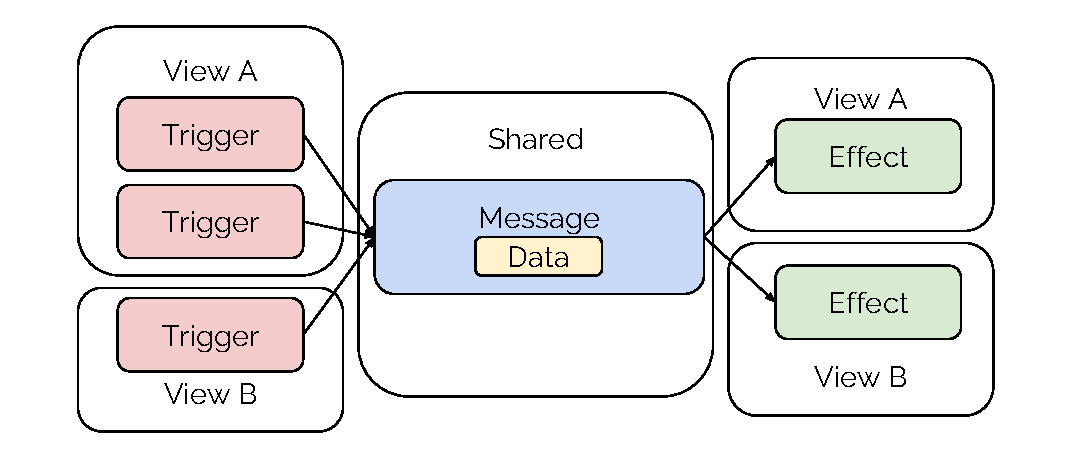
\includegraphics[width=\textwidth]{figures/concept/communication-pattern}
  \caption{%
    The message flow of the communication pattern:
    Every view can decide for itself whether to trigger an interaction or respond to an interaction with a visual effect.
  }\label{fig:concept:communication-pattern}
\end{figure}

Sometimes a visualization may not be able to interpret an interaction.
E.g.\ a bar chart can re-arrange the bars along the x-axis in case of a \emph{Reconfigure} interaction.
But a scatter plot constrains x- and y-coordinates of an entity on a certain data attribute.
Therefore, not only the \emph{trigger} and \emph{effect} is implementation specific, but also the handling of the interaction itself.

Every visualization decides on its own, how to react to a certain interaction.
That leads us to distinguishable, named interactions.
Every view can subscribe to certain interactions and receive messages in form of changed interaction types.
In order trigger an interaction, the visualization simply publishes to the named interaction.

This pattern is known as the \emph{Publish-subscribe pattern} and widely used in message queues.
The term \emph{interaction} in our case is equivalent to the term \emph{channel} or \emph{topic} commonly used in message queues.

